\documentclass{beamer}


\usepackage[english]{babel}
\usepackage[utf8]{inputenc}
\usepackage{amsmath,amssymb,amsfonts,amsthm}
\usepackage{stmaryrd}
\usepackage{hyperref}  % automagically makes clickable references, table of contents
\usepackage{enumerate}
\usepackage{lipsum}
\usepackage{graphicx}
\usepackage{wrapfig}
\usepackage{pifont}
\usepackage{epigraph}

\usepackage{tikz}
\usetikzlibrary{matrix, fit, positioning, decorations.pathmorphing, decorations.pathreplacing}
\tikzset{
	edge/.style={thick, ->},
	table nodes/.style={
		rectangle,
		draw=black,
		style=thick,
		align=center,
		minimum height=7mm,
		text depth=0.5ex,
		text height=2ex,
		inner xsep=0pt,
		outer sep=0pt,
		inner sep=0pt
	},
	table/.style={
		matrix of nodes,
		row sep=-0.5pt,
		column sep=-0.5pt,
		nodes={
			table nodes
		}
	}
}


% Sets and set operations
\newcommand{\R}{\mathbb{R}} % the reals
\newcommand{\Z}{\mathbb{Z}} % the integers
\newcommand{\N}{\mathbb{N}} % the natural numbers
\renewcommand{\O}[1]{\mathcal{O}\l(#1\r)}
%\newcommand{\pot}[1]{\mathcal{P}(#1)} % power set

% Other operators
%\renewcommand{\mod}{\operatorname{\%}}
\newcommand{\s}{\ast}

% Convenience
\renewcommand{\l}{\left} % short left
\renewcommand{\r}{\right} % short right
\newcommand{\pfrac}[2]{\l( \frac{#1}{#2} \r)}
\newcommand{\divmod}{\overset{\operatorname{divmod}}{\longrightarrow}}
\newcommand{\code}[1]{\texttt{#1}}


\newcommand{\trienode}[2]{% node label, options for matrix
	\matrix (n#1) [table, text width=7mm, ampersand replacement=\&, #2]
	{ #1 \& {} \& {} \& {} \& {} \\};
	\node[font=\tiny, anchor=south] at (n#1-1-2.north) {0};
	\node[font=\tiny, anchor=south] at (n#1-1-3.north) {1};
	\node[font=\tiny, anchor=south] at (n#1-1-4.north) {2};
	\node[font=\tiny, anchor=south] at (n#1-1-5.north) {3}
}


\newcommand{\itemspacing}[1]{\setlength\itemsep{#1}}

%\setbeamertemplate{bibliography item}{\insertbiblabel}
\setbeamertemplate{footline}[frame number]




\title{Storing a Sparse Table}
\subtitle{Seminar Theory of Efficient Hashing Techniques}
\date{21.07.2016}
\author{Simon Feiden}


\begin{document}
	
	
\maketitle

\begin{frame}
	\tableofcontents
\end{frame}


\section{Introduction}
\begin{frame}
	\frametitle{}
	\begin{itemize}
		\item Hello World
	\end{itemize}
\end{frame}



\section{Tries}
\begin{figure}
	\centering
%	\includegraphics[width=\textwidth]{topic/imgtries/sampletrie_drawn_transp}
	\newcommand{\trienode}[2]{% node label, options for matrix
	\matrix (n#1) [table, text width=7mm, ampersand replacement=\&, #2]
	{ #1 \& {} \& {} \& {} \& {} \\};
	\node[font=\tiny, anchor=south] at (n#1-1-2.north) {0};
	\node[font=\tiny, anchor=south] at (n#1-1-3.north) {1};
	\node[font=\tiny, anchor=south] at (n#1-1-4.north) {2};
	\node[font=\tiny, anchor=south] at (n#1-1-5.north) {3}
}

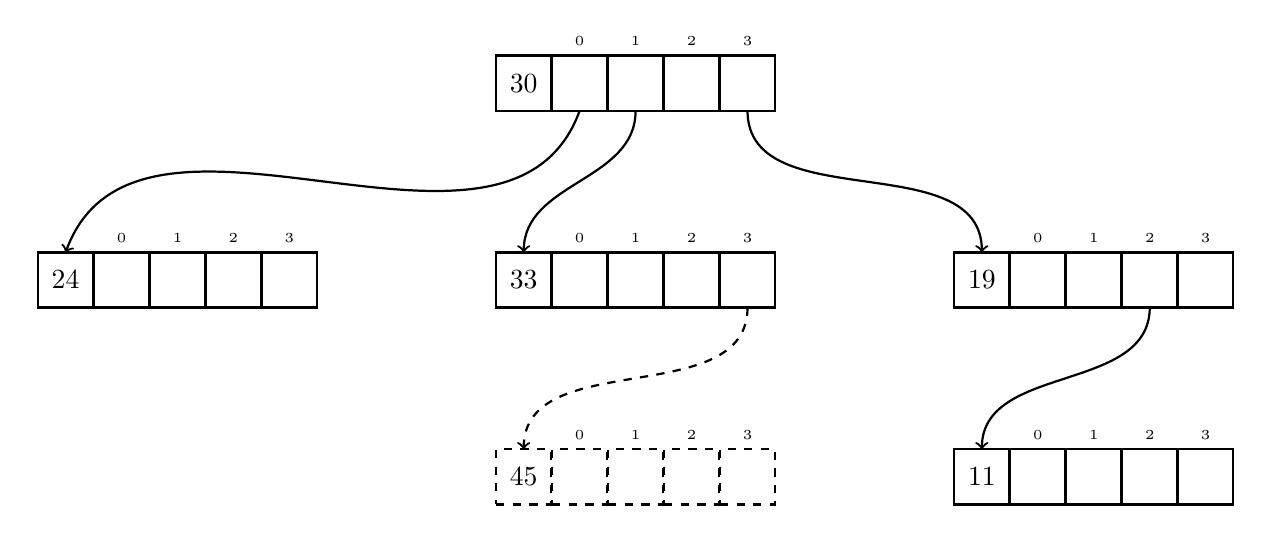
\begin{tikzpicture}[align=center, node distance=2.5cm]
	\trienode{30}{};	
	\trienode{33}{below of=n30};
	\trienode{24}{left =2cm of n33};
	\trienode{19}{right=2cm of n33};
	\trienode{11}{below of=n19};
	
	\trienode{45}{below of=n33, dashed};
	
	\draw[edge] (n30-1-2.south) to[out=250, in=70] (n24-1-1.north);
	\draw[edge] (n30-1-3.south) to[out=270, in=90] (n33-1-1.north);
	\draw[edge] (n30-1-5.south) to[out=270, in=90] (n19-1-1.north);
	\draw[edge] (n19-1-4.south) to[out=270, in=90] (n11-1-1.north);
	
	\draw[edge, dashed] (n33-1-5.south) to[out=270, in=90] (n45-1-1.north);
\end{tikzpicture}
	\caption{ \small A trie with $k = 4$ and entries 30, 24, 33, 19 and 11.
		To insert 45, we repeatedly divide 45 by 4, giving
			$45 \overset{1}{\longrightarrow} 11  \overset{3}{\longrightarrow} 2$.
		The remainders 1 and 3 lead to 33 where we insert a new node at slot 3 with value 45 as indicated.
		To delete 19, we search for it with the sequence $19 \overset{3}{\longrightarrow} 4$.
		Then, we localise a leaf that is a descendant of 19, in this trie, only 11 is possible.
		We remove 11 and set the value of 19 to 11.
		\label{fig:trie}}
\end{figure}


A trie \cite{knuth:tries} is a data structure.
In fact, a trie is a tree with the same maximum branching factor $k$ for all nodes.
A trie differs from balanced binary trees or other types of trees in the way that elements are inserted, looked up and deleted.
Every node of a trie contains an integer and $k$ pointers to its child nodes, indexed from 0 through $k - 1$.
Typically, $k$ is a power of 2.
The pointers in every node are \emph{null} initially and may be set when new elements are added.
The first element that is added to an empty trie is stored in the root and no new nodes are created.
Subsequent elements are added as follows:
Given a new element $e$, we repeatedly divide $e$ by $k$.
This gives a sequence of quotients and remainders.
Since the remainders are in the range 0 through $k - 1$, they specify a sequence of pointers.
The sequence starts at the root and descends one level into the tree with every step.
We follow the sequence of pointers until we reach a null pointer, which is where we insert a new node with value $e$.
This completes the insertion of a value into a trie.
Searching a value $v$ in a trie happens in a similar way:
First, we check for $v$ in the root.
If $v$ is not present there we follow the sequence of remainders as above.
At every node we check if it contains $v$.
If we eventually reach a null pointer the trie does not contain $v$, otherwise it does.
To delete a value $u$, we first search for $u$ in the trie and store the node $n_u$ which contains $u$.
If $n_u$ is a leaf, we simply delete it.
Otherwise, we locate any leaf that is a descendant of $n_u$, replace the value in $n_u$ by the leaf's value and then remove the leaf from the trie.
Examples for the operations can be found in Figure~\ref{fig:trie}.
A trie requires $\O{kn}$ space in the worst case.
The longest path starting at the root node in a trie has length $\O{\log_k N}$.
This means that search, insertion and deletion in a trie have the same time complexity:
During each operation, we follow some path in the trie.
In the worst case, the path is the longest in the trie and we follow it until we reach a leaf which requires $\O{\log_k N}$ time.
Insertion and deletion additionally manipulate some nodes, but in both cases these changes are constant time because only one or two nodes must be changed.
%If the values to be inserted into a trie are uniformly and independently distributed, lookup and insertion time are $\O{1}$.



\section{Tables and Displacements}
\begin{frame}{Sparse Tables}
	\begin{itemize}[<+->]
		\itemspacing{20pt}
		\item Tables are 2d-arrays with cells $\{1, \ldots, m\} \times \{1, \ldots, m\}$ % or $\{ 1, \ldots, m^2 \}$
		\item $N$ must be the table size
		\item Square tables $\implies$ $N = m \cdot m$
		\item Sparseness: $N \in \O{n^c}$
		\item Goal: compressing a table
	\end{itemize}
\end{frame}

\begin{frame}{Sparse Tables --- Displacements}
		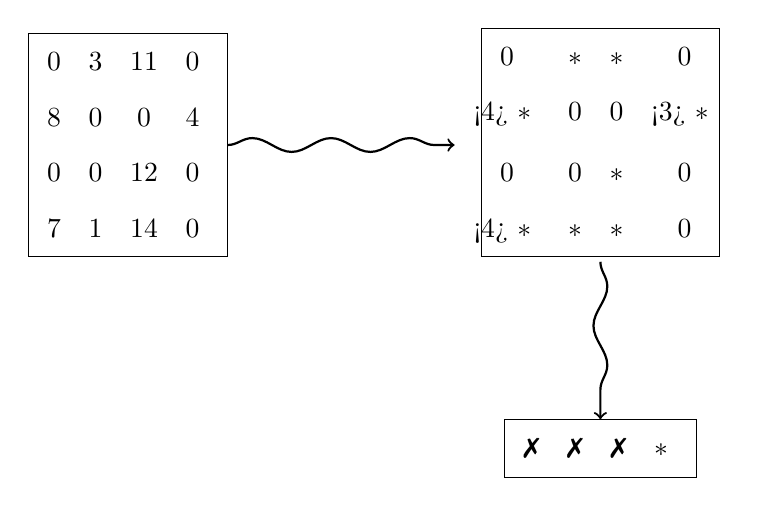
\begin{tikzpicture}[align=center, node distance=6cm]
			\matrix (tbl) [
				matrix of nodes,
				draw=none,
				row sep = 0.7em,
				column sep = 0em,
				ampersand replacement=\&
			] {
				0 \& 3 \& 11 \& 0 \\
				8 \& 0 \&  0 \&  4 \\
				0 \& 0 \& 12 \& 0 \\
				7 \& 1 \& 14 \&  0 \\
			};
			\node[draw, fit = (tbl-1-1) (tbl-4-4)] (tbl-fit) {};
			
			\uncover<2->{
				\matrix (tbl2) [
					matrix of nodes,
					draw=none,
					row sep = 0.7em,
					column sep = 0em,
					ampersand replacement=\&,
					right of = tbl
				] {
					0                 \& $\s$  \& $\s$ \&  0                 \\
					\alert<4>{ $\s$ } \& 0     \& 0    \&  \alert<3>{ $\s$ } \\
					0                 \& 0     \& $\s$ \&  0                 \\
					\alert<4>{ $\s$ } \& $\s$  \& $\s$ \&  0                 \\
				};
				\node[draw, fit = (tbl2-1-1) (tbl2-4-4)] (tbl2-fit) {};
				
				
				\draw[edge, decorate, decoration={snake, segment length = 10mm}] (tbl.east) to (tbl2.west);
			}
			
			\uncover<5->{
				\matrix (clash) [
				matrix of nodes,
				draw=none,
				row sep = 0.7em,
				column sep = 0em,
				ampersand replacement=\&,
				below = 2cm of tbl2
				] {
					\ding{55} \& \ding{55} \& \ding{55} \& $\s$   \\
				};
				\node[draw, fit = (clash-1-1) (clash-1-4)] (clash-fit) {};
				
				
				\draw[edge, decorate, decoration={snake, segment length = 10mm}] (tbl2.south) to (clash.north);
			}
		\end{tikzpicture}
\end{frame}

\begin{frame}{Sparse Tables --- Displacements}
	\centering
	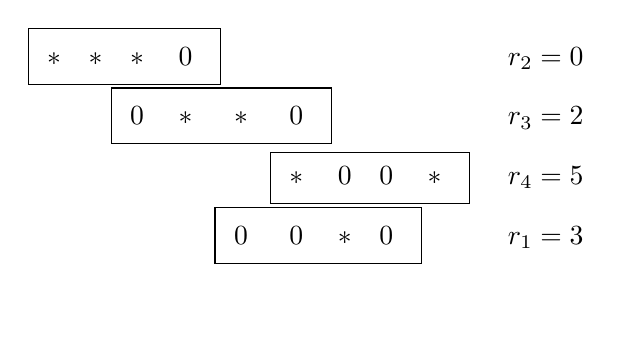
\begin{tikzpicture}[align=center, node distance=2cm]
		\matrix (mx) [%
			matrix of nodes,
			draw = none,
			row sep = 0.7em,
			column sep = 0em,
			ampersand replacement=\&
		] {
			$\s$ \& $\s$ \& $\s$ \& 0    \& {}   \& {}   \& {}   \& {} \& {}   \&[1em] $r_2 = 0$ \\
			{}   \& {}   \& 0    \& $\s$ \& $\s$ \& 0    \& {}   \& {} \& {}   \& $r_3 = 2$ \\
			{}   \& {}   \& {}   \& {}   \& {}   \& $\s$ \& 0    \& 0  \& $\s$ \& $r_4 = 5$ \\
			{}   \& {}   \& {}   \& {}   \& 0    \& 0    \& $\s$ \& 0  \& {}   \& $r_1 = 3$ \\
			$\phantom{5}$ \& $\phantom{6}$ \& $\phantom{7}$ \& $\phantom{10}$ \& $\phantom{11}$ \& $\phantom{13}$ \& $\phantom{3}$ \& $\phantom{0}$ \& $\phantom{16}$ \& $\phantom{r_1 = C}$ \\
		};
		
		\node[draw, fit = (mx-1-1) (mx-1-4)] (1-fit) {};
		\node[draw, fit = (mx-2-3) (mx-2-6)] (2-fit) {};
		\node[draw, fit = (mx-3-6) (mx-3-9)] (3-fit) {};
		\node[draw, fit = (mx-4-5) (mx-4-8)] (4-fit) {};
%		\node[draw, fit = (mx-5-1) (mx-5-9)] (C-fit) {};
	\end{tikzpicture}
	
	\begin{itemize} % placeholder for spacing for next frame
		\item[]
		\item[]
	\end{itemize}
\end{frame}

\begin{frame}{Row Displacements}
	\resizebox{\textwidth}{!}{
		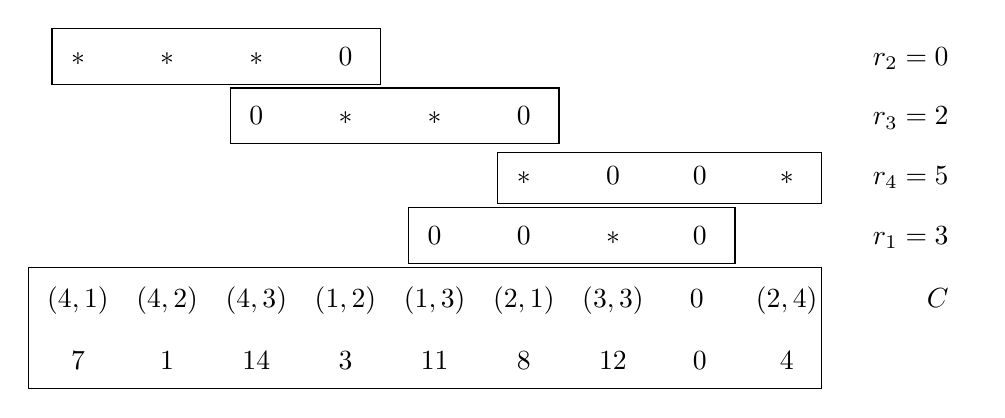
\begin{tikzpicture}[align=center, node distance=2cm]
			\matrix (mx) [%
				matrix of nodes,
				draw = none,
				row sep = 0.7em,
				column sep = 0em,
				ampersand replacement=\&
			] {
				$\s$ \& $\s$ \& $\s$ \& 0    \& {}   \& {}   \& {}   \& {} \& {}   \&[1em] $r_2 = 0$ \\
				{}   \& {}   \& 0    \& $\s$ \& $\s$ \& 0    \& {}   \& {} \& {}   \& $r_3 = 2$ \\
				{}   \& {}   \& {}   \& {}   \& {}   \& $\s$ \& 0    \& 0  \& $\s$ \& $r_4 = 5$ \\
				{}   \& {}   \& {}   \& {}   \& 0    \& 0    \& $\s$ \& 0  \& {}   \& $r_1 = 3$ \\
				$(4,1)$ \&
				$(4,2)$ \&
				$(4,3)$ \&
				$(1,2)$ \&
				$(1,3)$ \&
				$(2,1)$ \&
				$(3,3)$ \&
				$\phantom{(,}0\phantom{0)}$ \&
				$(2,4)$ \&
				$\phantom{r_1 = } C$ \\
				7 \& 1 \& 14 \& 3 \& 11 \& 8 \& 12 \&  0 \&  4 \\
			};
			
			\node[draw, fit = (mx-1-1) (mx-1-4)] (1-fit) {};
			\node[draw, fit = (mx-2-3) (mx-2-6)] (2-fit) {};
			\node[draw, fit = (mx-3-6) (mx-3-9)] (3-fit) {};
			\node[draw, fit = (mx-4-5) (mx-4-8)] (4-fit) {};
			\node[draw, fit = (mx-5-1) (mx-6-9)] (C-fit) {};
		\end{tikzpicture}
	}
	
	\begin{itemize}
		\item<2-> Finding optimal row displacements is NP-complete
		\item<3-> Heuristic approach: sort rows by number of nonnulls
	\end{itemize}
\end{frame}

\begin{frame}{Row Displacements}
	\begin{itemize}[<+->]
		\itemspacing{20pt}
		\item Essential operation on a table: \code{lookup} of key $k$
		\item Calculate position $(i, j)$ for $k$
		\item Check if $C(r_i + j)$ equals $k$
		\item $\O{1}$ lookup in $C$
		\item Single Displacements perform bad in worst case
	\end{itemize}
\end{frame}


\begin{frame}
	\begin{quotation}
		Any problem in computer science can be solved by another layer of indirection.
	\end{quotation}
	\vspace*{-1em}
	\begin{flushright}
		\textup{
		--- David Wheeler
		}
	\end{flushright}
\end{frame}


\section{RDI Compression}
\begin{frame}{RDI Compression}
	\centering
	\resizebox{!}{0.75\textheight}{
		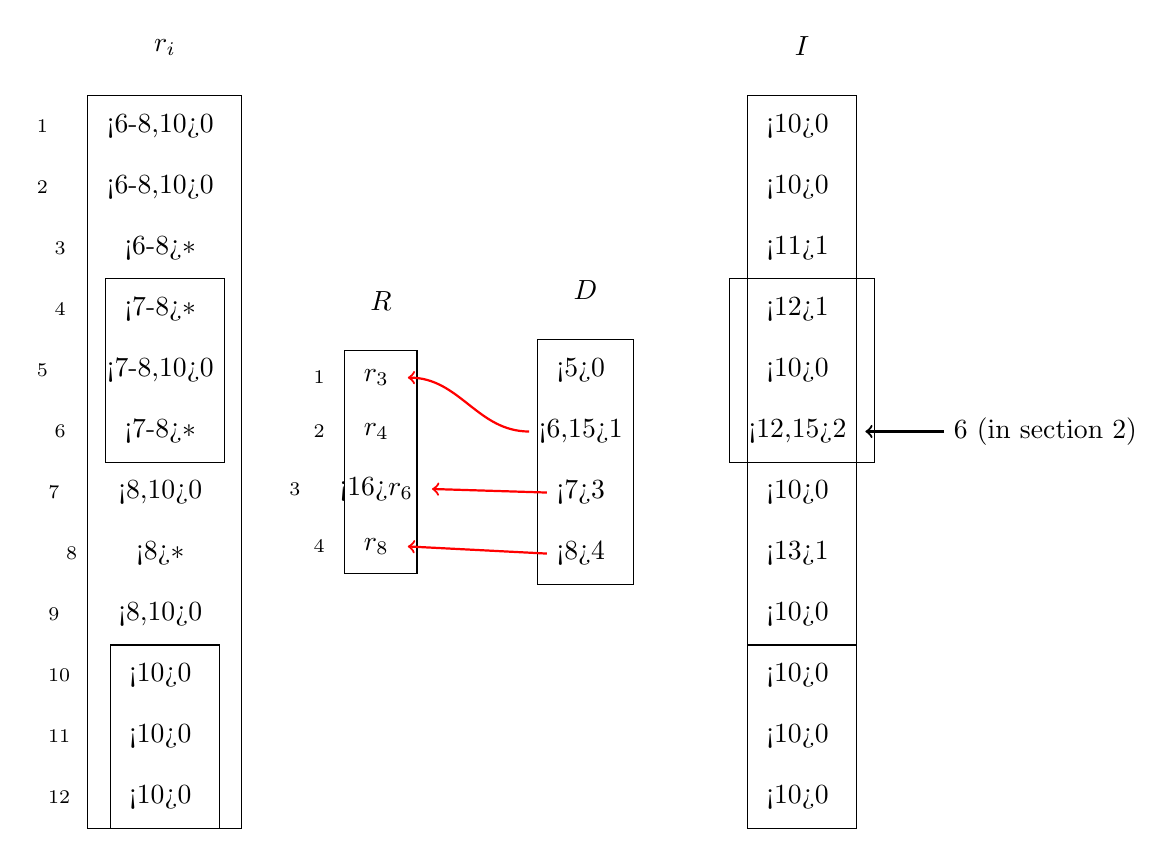
\begin{tikzpicture}[align=center, node distance=0.5cm and 1cm]
			\matrix (ri) [%
				matrix of nodes,
				draw = none,
				row sep = 0.7em,
				column sep = 0em
			]
			{
				\alert<6-8,10>{0}    \\
				\alert<6-8,10>{0}    \\
				\alert<6-8>{$\s$} \\
				\alert<7-8>{$\s$} \\
				\alert<7-8,10>{0}     \\
				\alert<7-8>{$\s$} \\
				\alert<8,10>{0}      \\
				\alert<8>{$\s$} \\
				\alert<8,10>{0}    \\
				\alert<10>{0}     \\
				\alert<10>{0}     \\
				\alert<10>{0}     \\
			};
			\node[draw, fit = (ri-1-1) (ri-12-1)] (ri-fit) {};
			\node[above = of ri-1-1] (rilabel) {$r_i$};
			
			\foreach \n in {1,...,12} {
				\node[font=\scriptsize, left = 0.5cm of ri-\n-1 ] {\n};
			}
			
			\visible<2->{
				\matrix (R) [%
					matrix of nodes,
					draw = none,
					row sep = 0.7em,
					column sep = 0em,
					right = of ri
				]
				{
					$r_3$ \\ $r_4$ \\ \alert<16>{$r_6$} \\ $r_8$ \\
				};
				\node[draw, fit = (R-1-1) (R-4-1)] (r-fit) {};
				\node[above = of R-1-1] (Rlabel) {$R$};
				
				\foreach \n in {1,...,4} {
					\node[font=\scriptsize, left = 0.25cm of R-\n-1 ] {\n};
				}
			}
			
			
			\visible<3->{
				\node[draw, fit = (ri-4-1) (ri-6-1)] (c) {};
				\node[draw, fit = (ri-10-1) (ri-12-1)] (d) {};
			}
			
			
			\visible<4->{
				\matrix (D) [%
					matrix of nodes,
					draw = none,
					row sep = 0.7em,
					column sep = 0em,
					right = of R
				]
				{
					\alert<5>{0} \\
					\alert<6,15>{1} \\
					\alert<7>{3} \\
					\alert<8>{4} \\
				};
				\node[draw, fit = (D-1-1) (D-4-1)] (D-fit) {};
				\node[above = of D-1-1] (Dlabel) {$D$};
			}
			
			\visible<6>{
				\draw[edge, red] (D-2-1.west) to[out=180, in=0] (R-1-1.east);
			}
				
			\visible<7>{
				\draw[edge, red] (D-3-1.west) to (R-3-1.east);
			}
				
			\visible<8>{
				\draw[edge, red] (D-4-1.west) to (R-4-1.east);
			}
			
			
			\visible<9->{
				\matrix (I) [%
					matrix of nodes,
					draw = none,
					row sep = 0.7em,
					column sep = 0em,
					right = of D
				]
				{
					\alert<10>{0} \\
					\alert<10>{0} \\
					\alert<11>{1} \\
					\alert<12>{1} \\
					\alert<10>{0} \\
					\alert<12,15>{2} \\
					\alert<10>{0} \\
					\alert<13>{1} \\
					\alert<10>{0} \\
					\alert<10>{0} \\
					\alert<10>{0} \\
					\alert<10>{0} \\
				};
				
				\node[draw, fit = (I-1-1) (I-12-1)] (i-fit) {};
				\node[above = of I-1-1] (Ilabel) {$I$};
				
				
				
				\node[draw, fit = (I-4-1) (I-6-1)] (a) {};
				\node[draw, fit = (I-10-1) (I-12-1)] (b) {};
			}
			
			
			\visible<14->{
				\node[right = 1cm of I-6-1] (lu6) {6 (in section 2)};
				\draw[edge] (lu6.west) to (I-6-1.east);
			}
			
		\end{tikzpicture}
	}
\end{frame}

\begin{frame}{RDI Compression}
	\begin{itemize}[<+->]
		\itemspacing{20pt}
		\item Values in $I$ are in $\O{\log \log n}$
		\item Pack multiple small values into one
		\item Reduces required storage for $I$
		\item Achieves overall compression of row displacements
	\end{itemize}
\end{frame}


\section{Combining Tries and Tables}
%Having introduced tries and the displacement storage scheme, we can now combine both.
Recall that $N$ is the greatest name that we want to store in our table and $n$ is the number of entries we want to store.
In the beginning, we required that $N$ is bounded by a polynomial of $n$ for both the tries and the displacement scheme.
To overcome this restriction and provide a storage scheme that works well for arbitrary values of $n$ and $N$, we can combine tries and the displacement scheme.
Since we still consider the static case of storage and lookup, we know which values we have to store.
The first step is to insert all these values into a trie with branching factor $n$.
The trie then contains $n$ nodes with $n$ pointers each.
Note that of these $n^2$ pointers, exactly $n - 1$ are nonnull, since every node except the root is pointed at exactly once.
The pointer arrays of each node can be combined into a table of size $n \times n$ and compressed using double displacements (with $m = n$) and a displacement directory.
The properties of the trie data structure combined with the compression methods finally give us a method with storage in $\O{n}$ and access time in $\O{\log_n N}$.



\begin{frame}
	\frametitle{\ }
	\begin{center}
		\LARGE Thank you for your attention!
	\end{center}
\end{frame}


\begin{frame}
	% empty frame
\end{frame}


\input{bounds/more.tex}


\bibliographystyle{alpha}
\bibliography{literature}


\end{document}

